\problem{}
\subproblem{}
فرض کنیم نقاط $x_1,x_2,...,x_n$ را داریم به صورتی که $x_i$ ها نقاط $quantile$ ها هستند.
داریم \\
\[\frac{1}{n} = \int_{a}^{b} f(x)dx = P(a<X<b) = P(a<\sigma Y +\mu<b) = P(\frac{a-\mu}{\sigma}<Y<\frac{b-\mu}{\sigma}) = \int_{\frac{a-\mu}{\sigma}}^{\frac{b-\mu}{\sigma}} f(y)dy\]\\
که $a = x_i$ و $b = x_{i+1}$.\\\\
پس نقطه متناظر $x_i$   در نمودار توزیع$X$ برابر است با $\frac{x_i-\mu}{\sigma}$ که این یعنی با رسم نمودار 
qqplot برای این دو متغیر نقاط روی یه خط صاف با شیب $\frac{1}{\sigma}$ و عرض از مبدا $-\frac{\mu}{\sigma}$ داریم.
\begin{figure}[H]
	\centering
	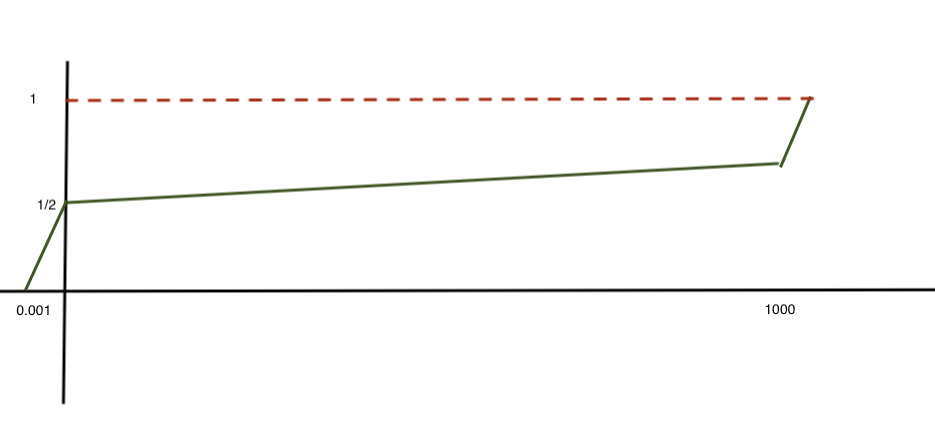
\includegraphics[width=0.5\textwidth]{/Users/kajal/Documents/statistics/resources/hw2/Figure_5.png}
\end{figure}
\subproblem{}
کد پایتون:
\begin{figure}[H]
	\centering
	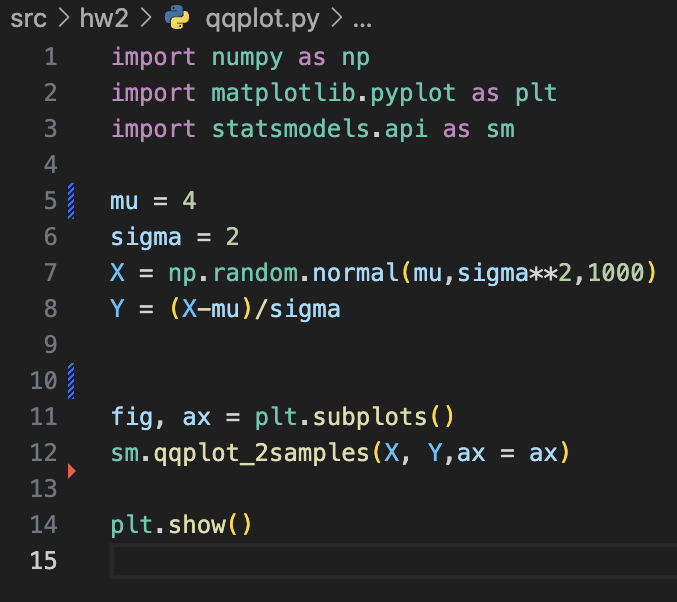
\includegraphics[width=0.5\textwidth]{/Users/kajal/Documents/statistics/resources/hw2/Figure_6.png}
\end{figure}
خروجی:
\begin{figure}[H]
	\centering
	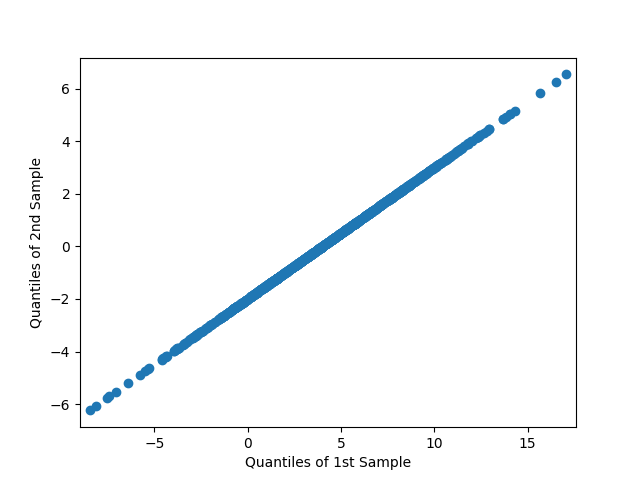
\includegraphics[width=0.5\textwidth]{/Users/kajal/Documents/statistics/resources/hw2/Figure_7.png}
\end{figure}